\chapter*{Appendix A: Working and representation of the descriptors}
\addcontentsline{toc}{chapter}{Appendix A: Working and representation of the descriptors}

\section*{Feature extraction}

Some feature extraction has already been provided.
In short, images are converted from there typical RGB representation to a numerical representation of interesting points, which can be used as input for our model.
How this is done and could be optimized is briefly discussed here since it consists of provided code for the Kaggle competition.

Instead of using the whole image as data, only a select few of \textit{interesting points} of the image are taken into consideration.
These interesting points of an image are often found by using the \emph{Shi-Tomasi corner detector}, but some descriptors have different implementations.
As the name suggests, these interesting points are \textit{strong corners on an image}.

Shown in figure \ref{fig:1-poi} is an example output of interesting points found by the Shi-Tomasi corner detector.
It's clear that its performance varies a lot, but finding interesting points isn't an easy task and thus the results are better then they might seem on first sight.
It's also noted that SIFT is used for the models in this report, which uses a different, patented, technique for interesting point detection.

\begin{figure*}[ht]
    \centering
    \begin{subfigure}{.35\textwidth}
        \centering
        \fbox{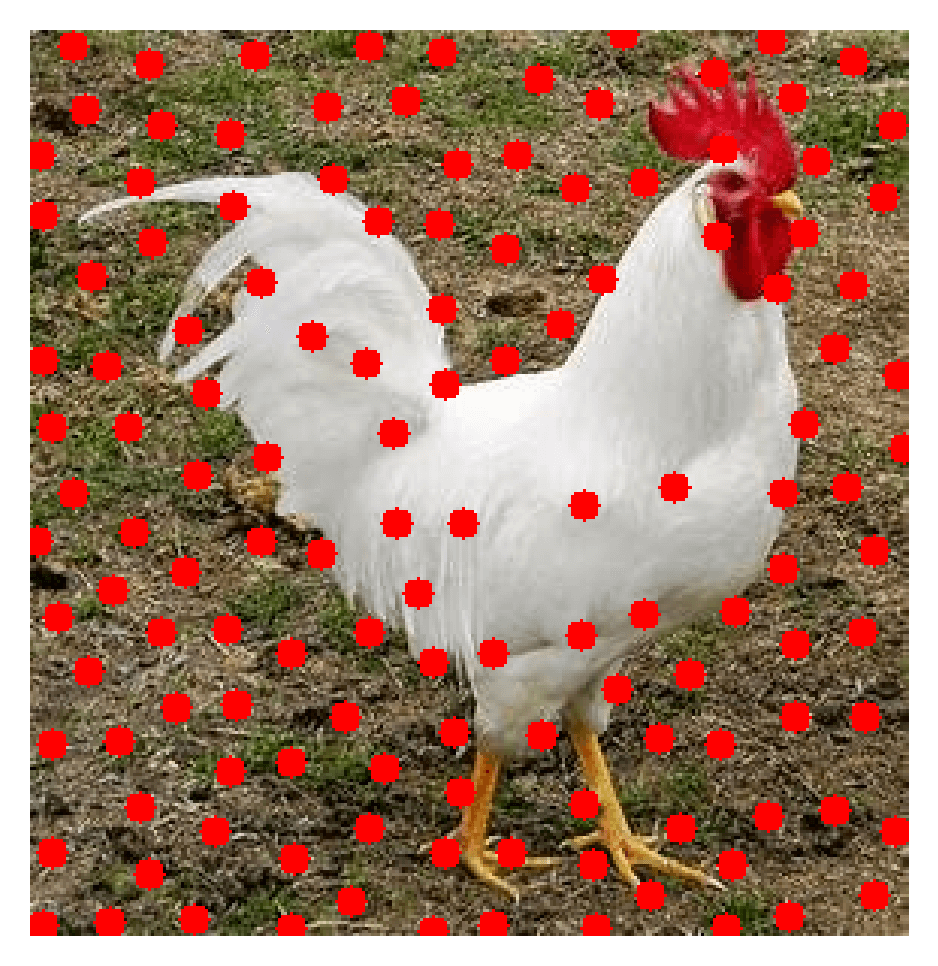
\includegraphics[width=0.9\textwidth]{images/1/1-data_analysis-POI_chicken.png}}
        \captionsetup{width=0.9\linewidth}
        \captionsetup{justification=centering}
        \caption{First chicken in data.}
    \end{subfigure}
    \hspace{1cm}
    \begin{subfigure}{.52\textwidth}
        \centering
        \fbox{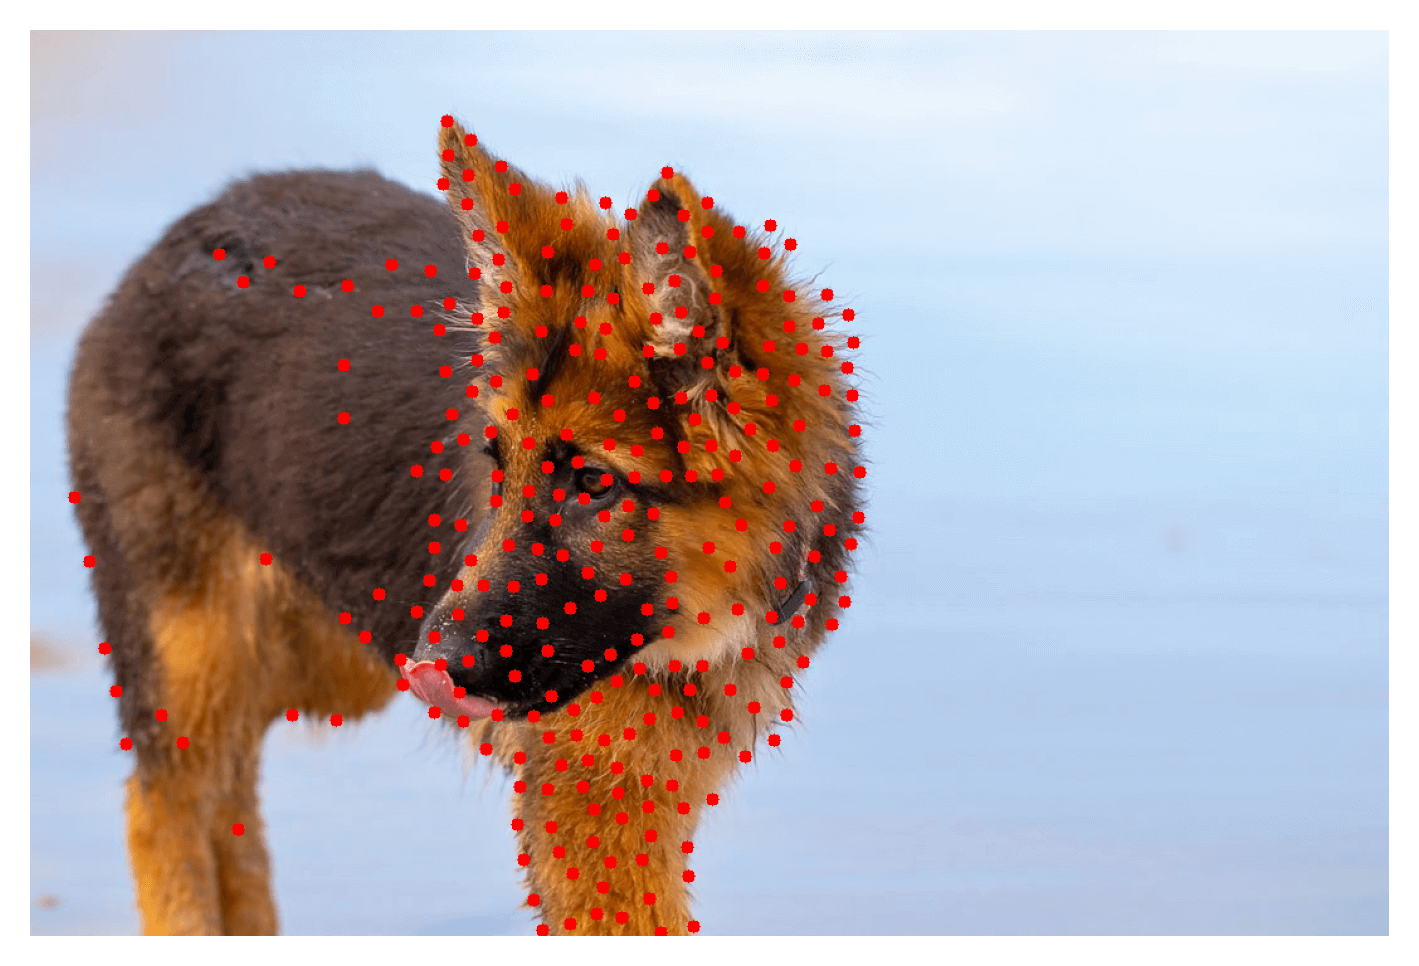
\includegraphics[width=0.9\textwidth]{images/1/1-data_analysis-POI_german_shepherd.png}}
        \captionsetup{width=0.9\linewidth}
        \captionsetup{justification=centering}
        \caption{First German shepherd in train data}
    \end{subfigure}
    \captionsetup{width=0.8\linewidth}
    \captionsetup{justification=centering}
    \caption{Points of interest found by the Shi-Tomasi corner detector.}
    \label{fig:1-poi}
\end{figure*}


%------------------------------------

\section*{The numerical representation}

These interesting points now need to be represented by numerical values that have actual meaning.
Remember from section \ref{section:DA_deeper_look_data} that the provided images differ a lot.
Thus the numerical representation, generated by a descriptor, has to be so that it minifies the impact of different lighting, scaling...
afterwards, these values can be clustered together using the \texttt{createCodebook} function which uses Mini-Batch K-Means clustering.
This could also benefit from fine-tuning.

An overview showing histograms for each word (cluster) and a corresponding correlation matrix when opting for SIFT with 30 clusters is shown in figure \ref{fig:1-cm}.
It is visible that the values are normalized.
This would have to be checked for all descriptors used and perhaps some outliers would need to be removed.
The correlation between these clusters doesn't seem too dramatic in this case ($|$correlation value$| \neq 1 $).
A low correlation between clusters is mostly positive for model building since it suggests each cluster represent a distinct concept.
This is again something that would have to be checked for different parameters.

\begin{figure}[H]
    \centering
    \begin{subfigure}{.45\textwidth}
        \centering
        \fbox{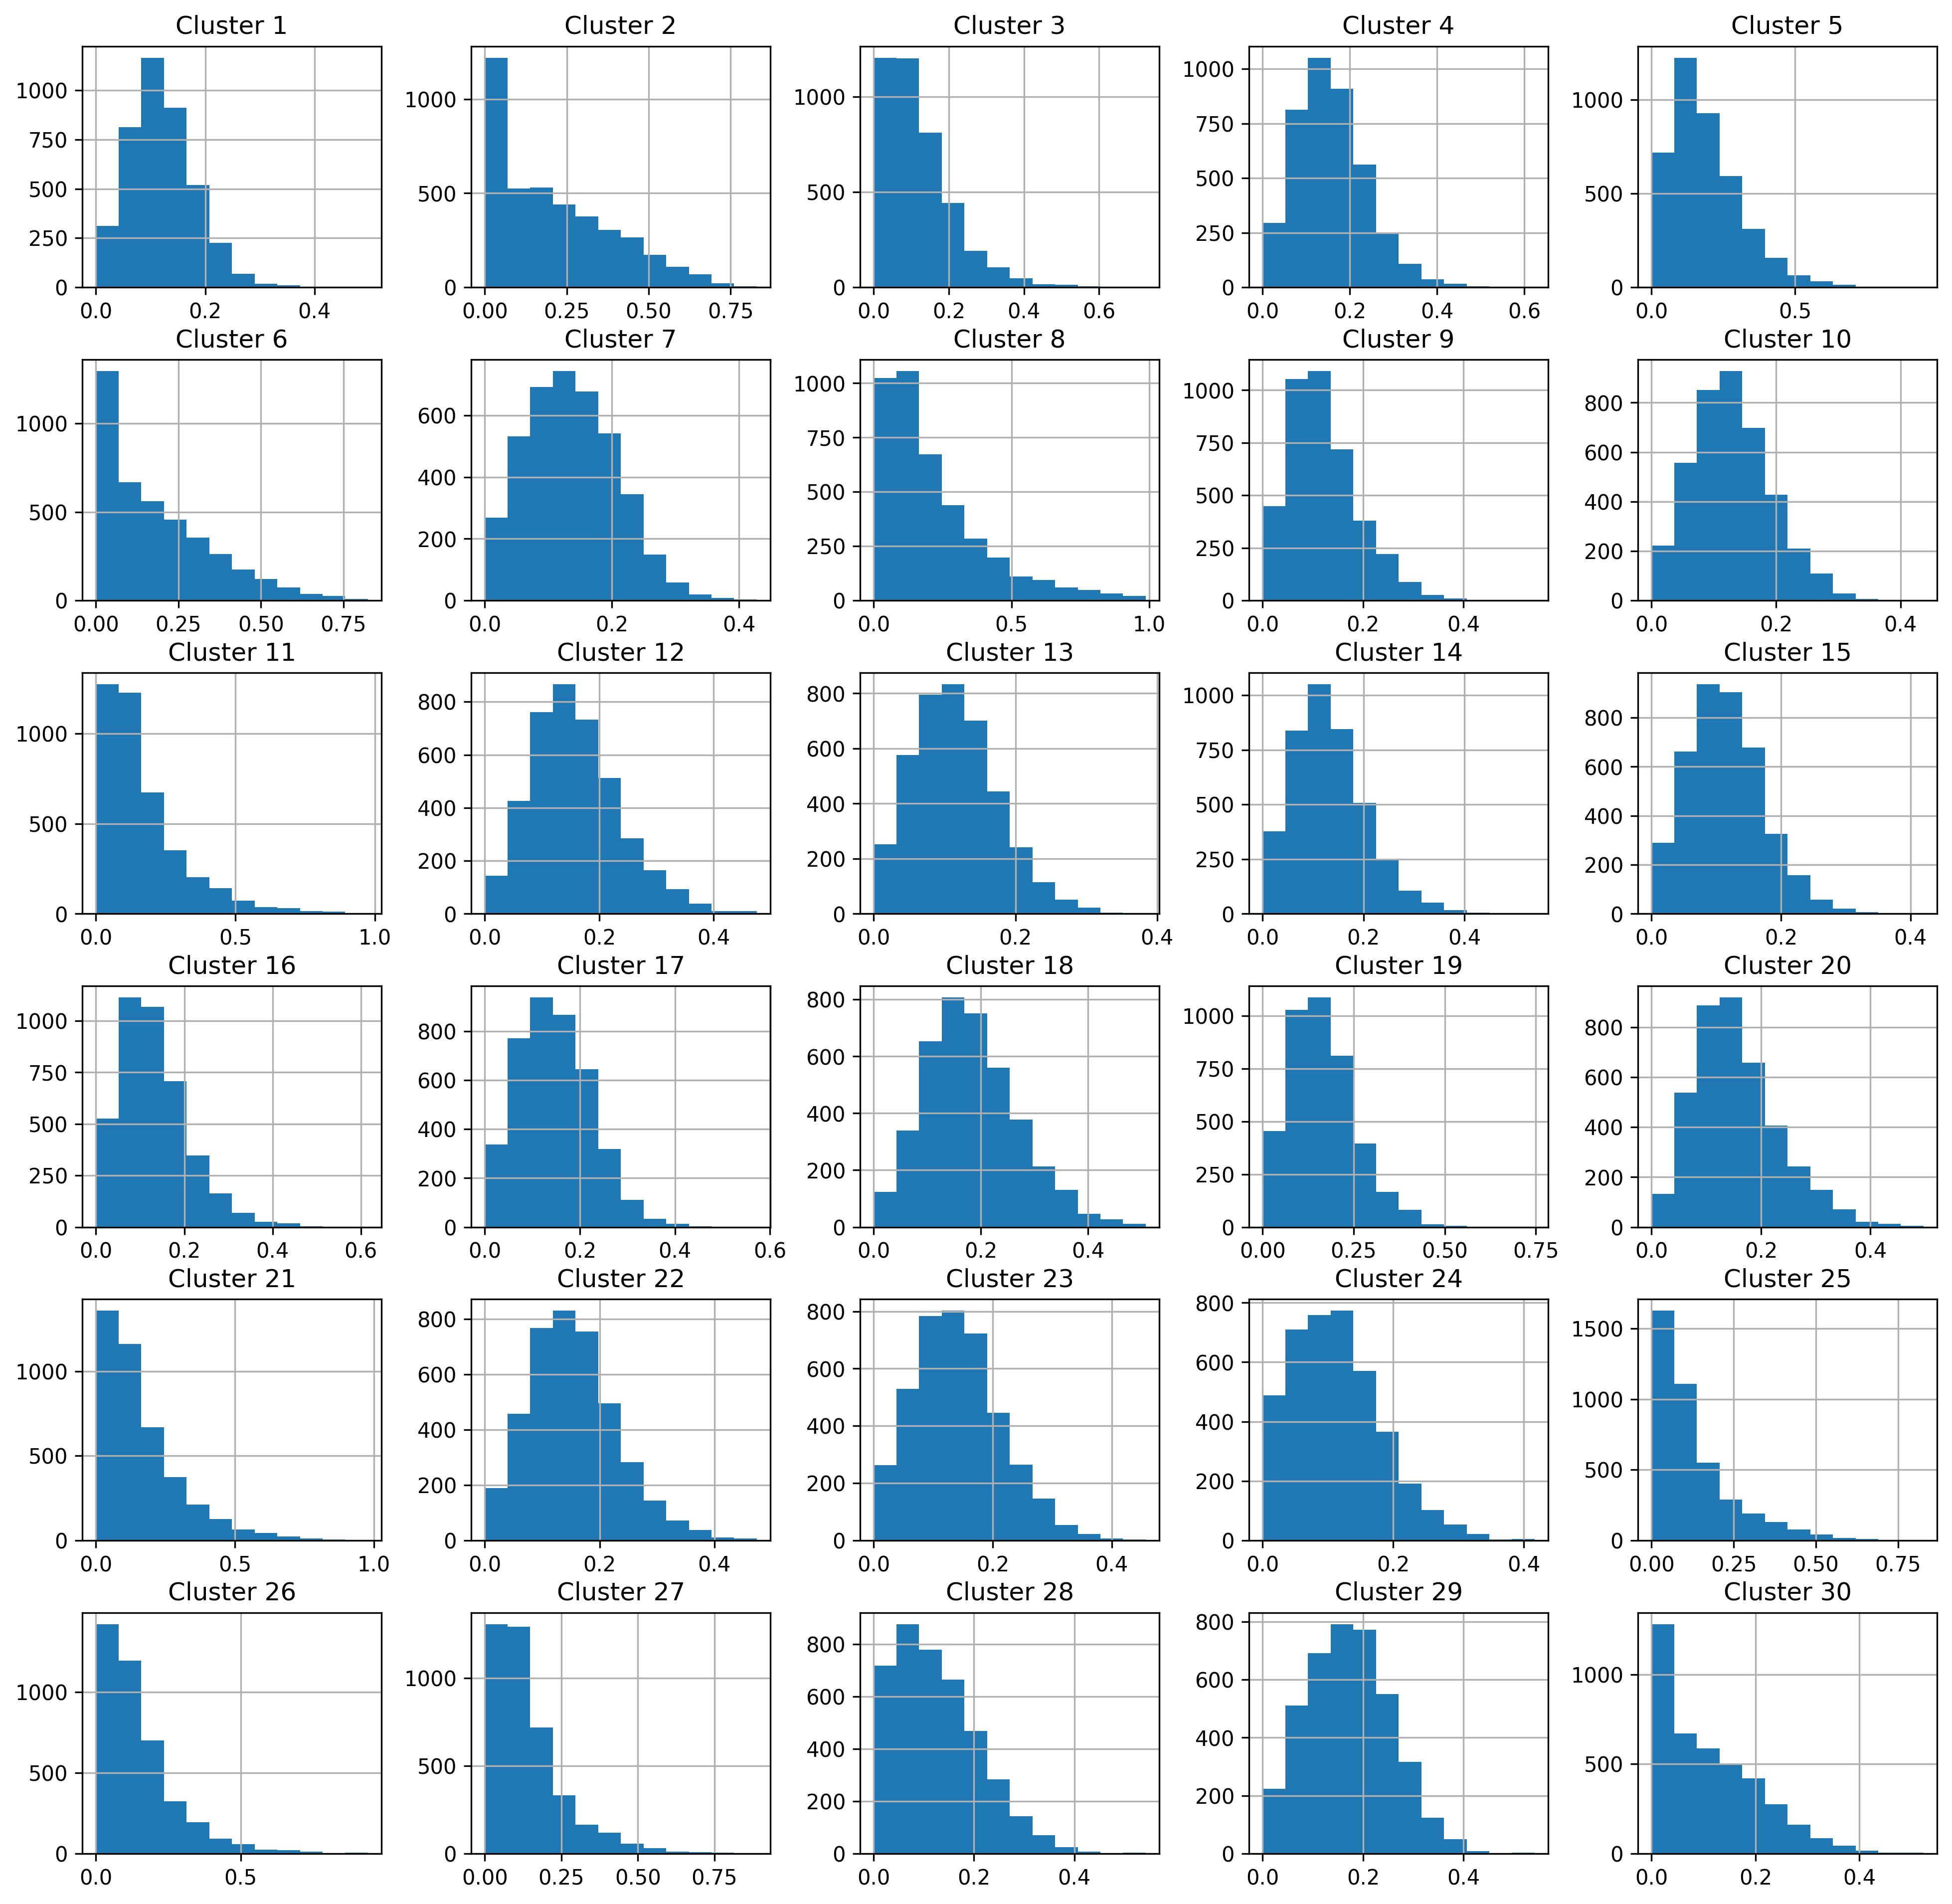
\includegraphics[width=0.7\textwidth]{images/1/1-data_analysis-feature_representation.png}}
        \captionsetup{width=0.9\linewidth}
        \captionsetup{justification=centering}
        \caption{Histogram for each cluster.}
    \end{subfigure}
    \hspace{1cm}
    \begin{subfigure}{.45\textwidth}
        \centering
        \fbox{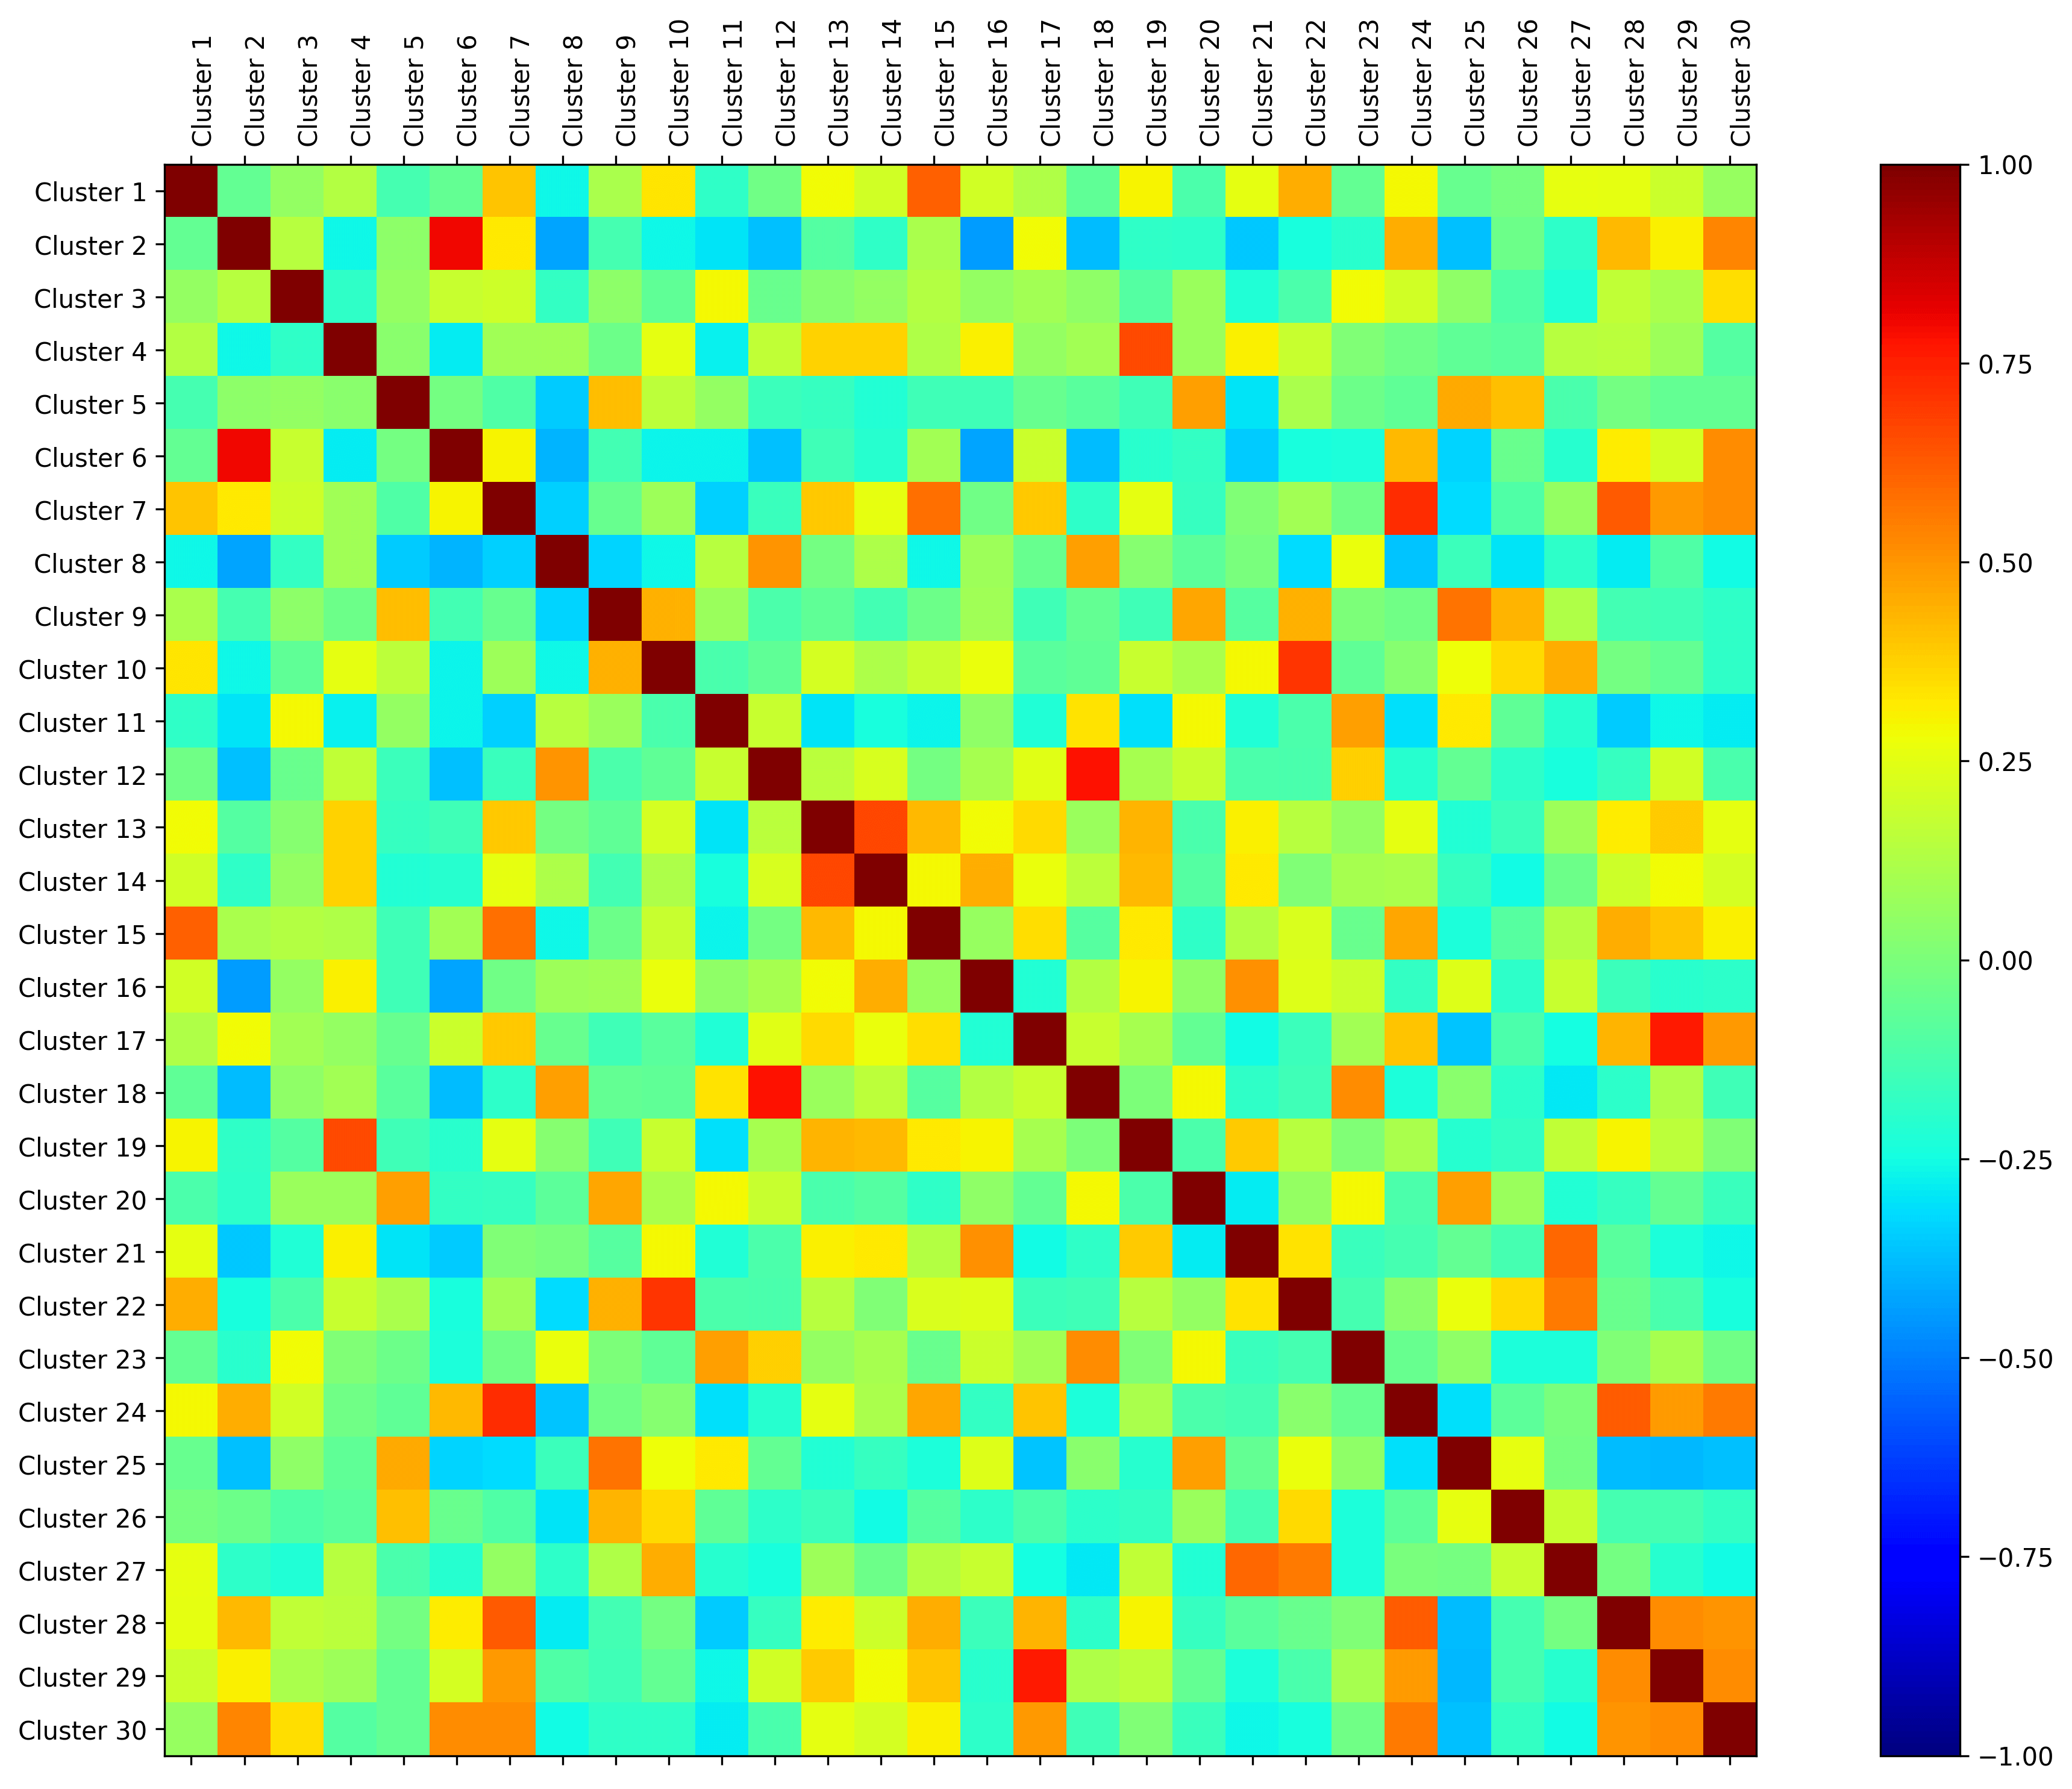
\includegraphics[width=0.8\textwidth]{images/1/1-data_analysis-correlation_matrix.png}}
        \captionsetup{width=0.9\linewidth}
        \captionsetup{justification=centering}
        \caption{Correlation matrix for all clusters.}
    \end{subfigure}
    \captionsetup{width=0.8\linewidth}
    \captionsetup{justification=centering}
    \caption{Data analysis of encoded images using SIFT with 30 clusters.}
    \label{fig:1-cm}
\end{figure}


%------------------------------------------------------------------------------------------------------------------------------------------------


\chapter*{Appendix B: Important LBM parameters}
\addcontentsline{toc}{chapter}{Appendix B: Important LBM parameters}

As found in the documentation of the \texttt{LogisticRegression} function available in the SciKit Learn library there are multiple (optional) parameters \citep{scikit_learn}.
The most interesting ones are:

\begin{itemize}
    \item \emph{solver}
    \begin{itemize}
        \item Specifies which solver should be used for the optimization problem in the model.
        \item \emph{lbfgs} is used as default and whilst a little slow, this parameter doesn't require further fine-tuning.
    \end{itemize}
    \item \emph{penalty}
    \begin{itemize}
        \item Since the \emph{lbfgs} solver is used, the default \emph{l2} penalization norm is the only one that can be used.
    \end{itemize}
    \item \emph{class\_weight}
    \begin{itemize}
        \item This parameter defaults to None but can be set to balanced to take into account the unbalance in our data, as discussed in section \ref{section:DA_data_distribution}.
        \item The results with this parameter set to balanced will be studied.
    \end{itemize}
    \item \emph{C}
    \begin{itemize}
        \item The regularisation hyperparameter C defaults to 1. Fine-tuning this could boost performance.
    \end{itemize}
    \item \emph{max\_iter}
    \begin{itemize}
        \item This parameter can be changed so that convergence might be found, which is not the case right now.
    \end{itemize}
    \item \emph{fit\_intercept}
    \begin{itemize}
        \item Boolean that specifies if a constant (a.k.a. bias or intercept) should be added to the decision function.
        \item The results with this parameter set to true and false should be checked.
    \end{itemize}
\end{itemize}

%------------------------------------------------------------------------------------------------------------------------------------------------